\section{Results}
\label{sec:results}

In this section, we present the fiducial constraints we obtain from the weak lensing cosmological inference in real space and compare them to other experiments and surveys. Measurements from this analysis are compared to other, comparable measurements in order to obtain precise joint constraints of the growth of structure. 

\begin{figure}[ht]
    \centering
    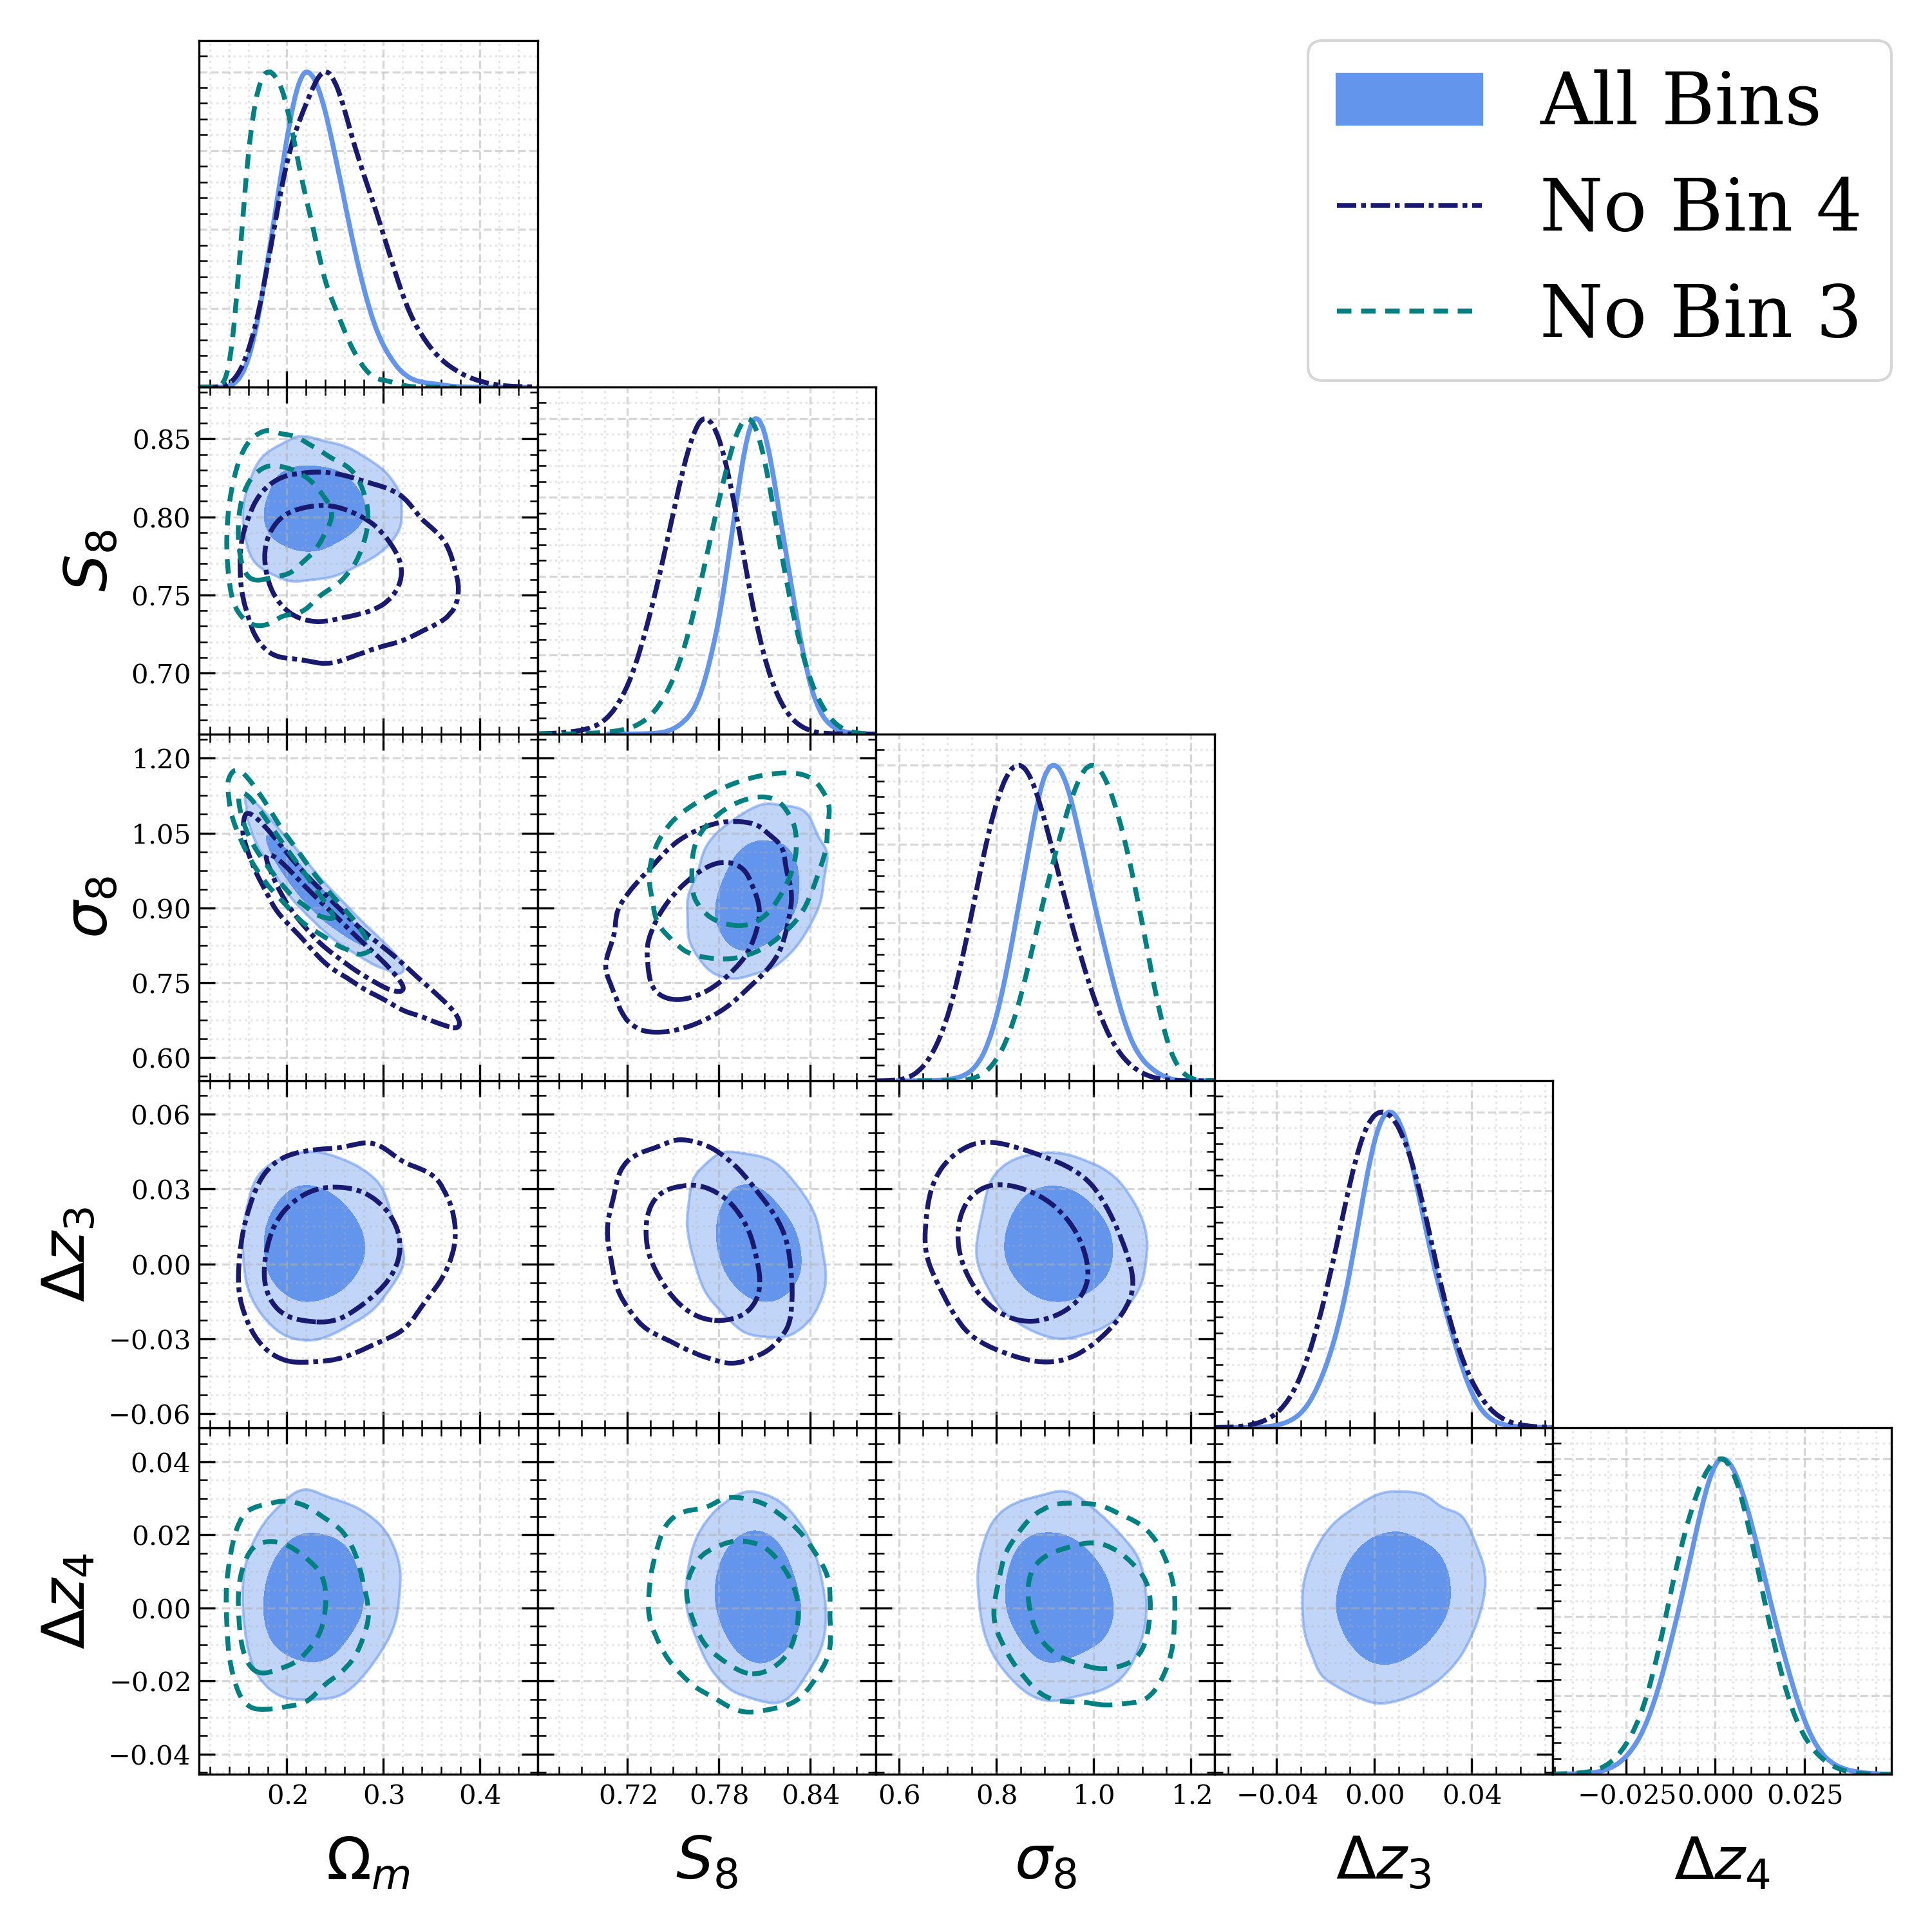
\includegraphics[width=0.9\textwidth]{img/corner_excluded_bins.png}
    \caption{To assess the robustness of the measurement, we exclude Bin 3 and Bin 4 respectively from the chain inference. The measurements are shown to be consistent between the two and consistent with the "All Bins" measurement.}
    \label{fig:corner_excluded_bins}
\end{figure}

Furthermore, we investigate the robustness of this analysis by comparing the results to importance sampling of the fiducial chains, as well as using different configuration for the tomographic $n(z)$ distributions. We note that following the setup proposed in \texttt{CosmoSIS}, the convention used for $\Delta z$ parameter shifts is opposed to the one presented in the clustering redshift analyses \cite{HSCClusteringRau2023, ChoppinDeJanvry2025a} and in the cosmological inference works such as \cite{Li2023_HSCY3_CosmicShear, Dalal2023CosmoShearHSC, Zhang2025aTomographic2x2pt, Zhang2025bTomographic3x2pt}. Here, a positive shift implies that the real $n(z)$ distribution is at higher redshifts than the original, calibrated one proposed in the redshift calibration analyses: the original convention implied the same for negative shifts.

\begin{figure}[ht]
    \centering
    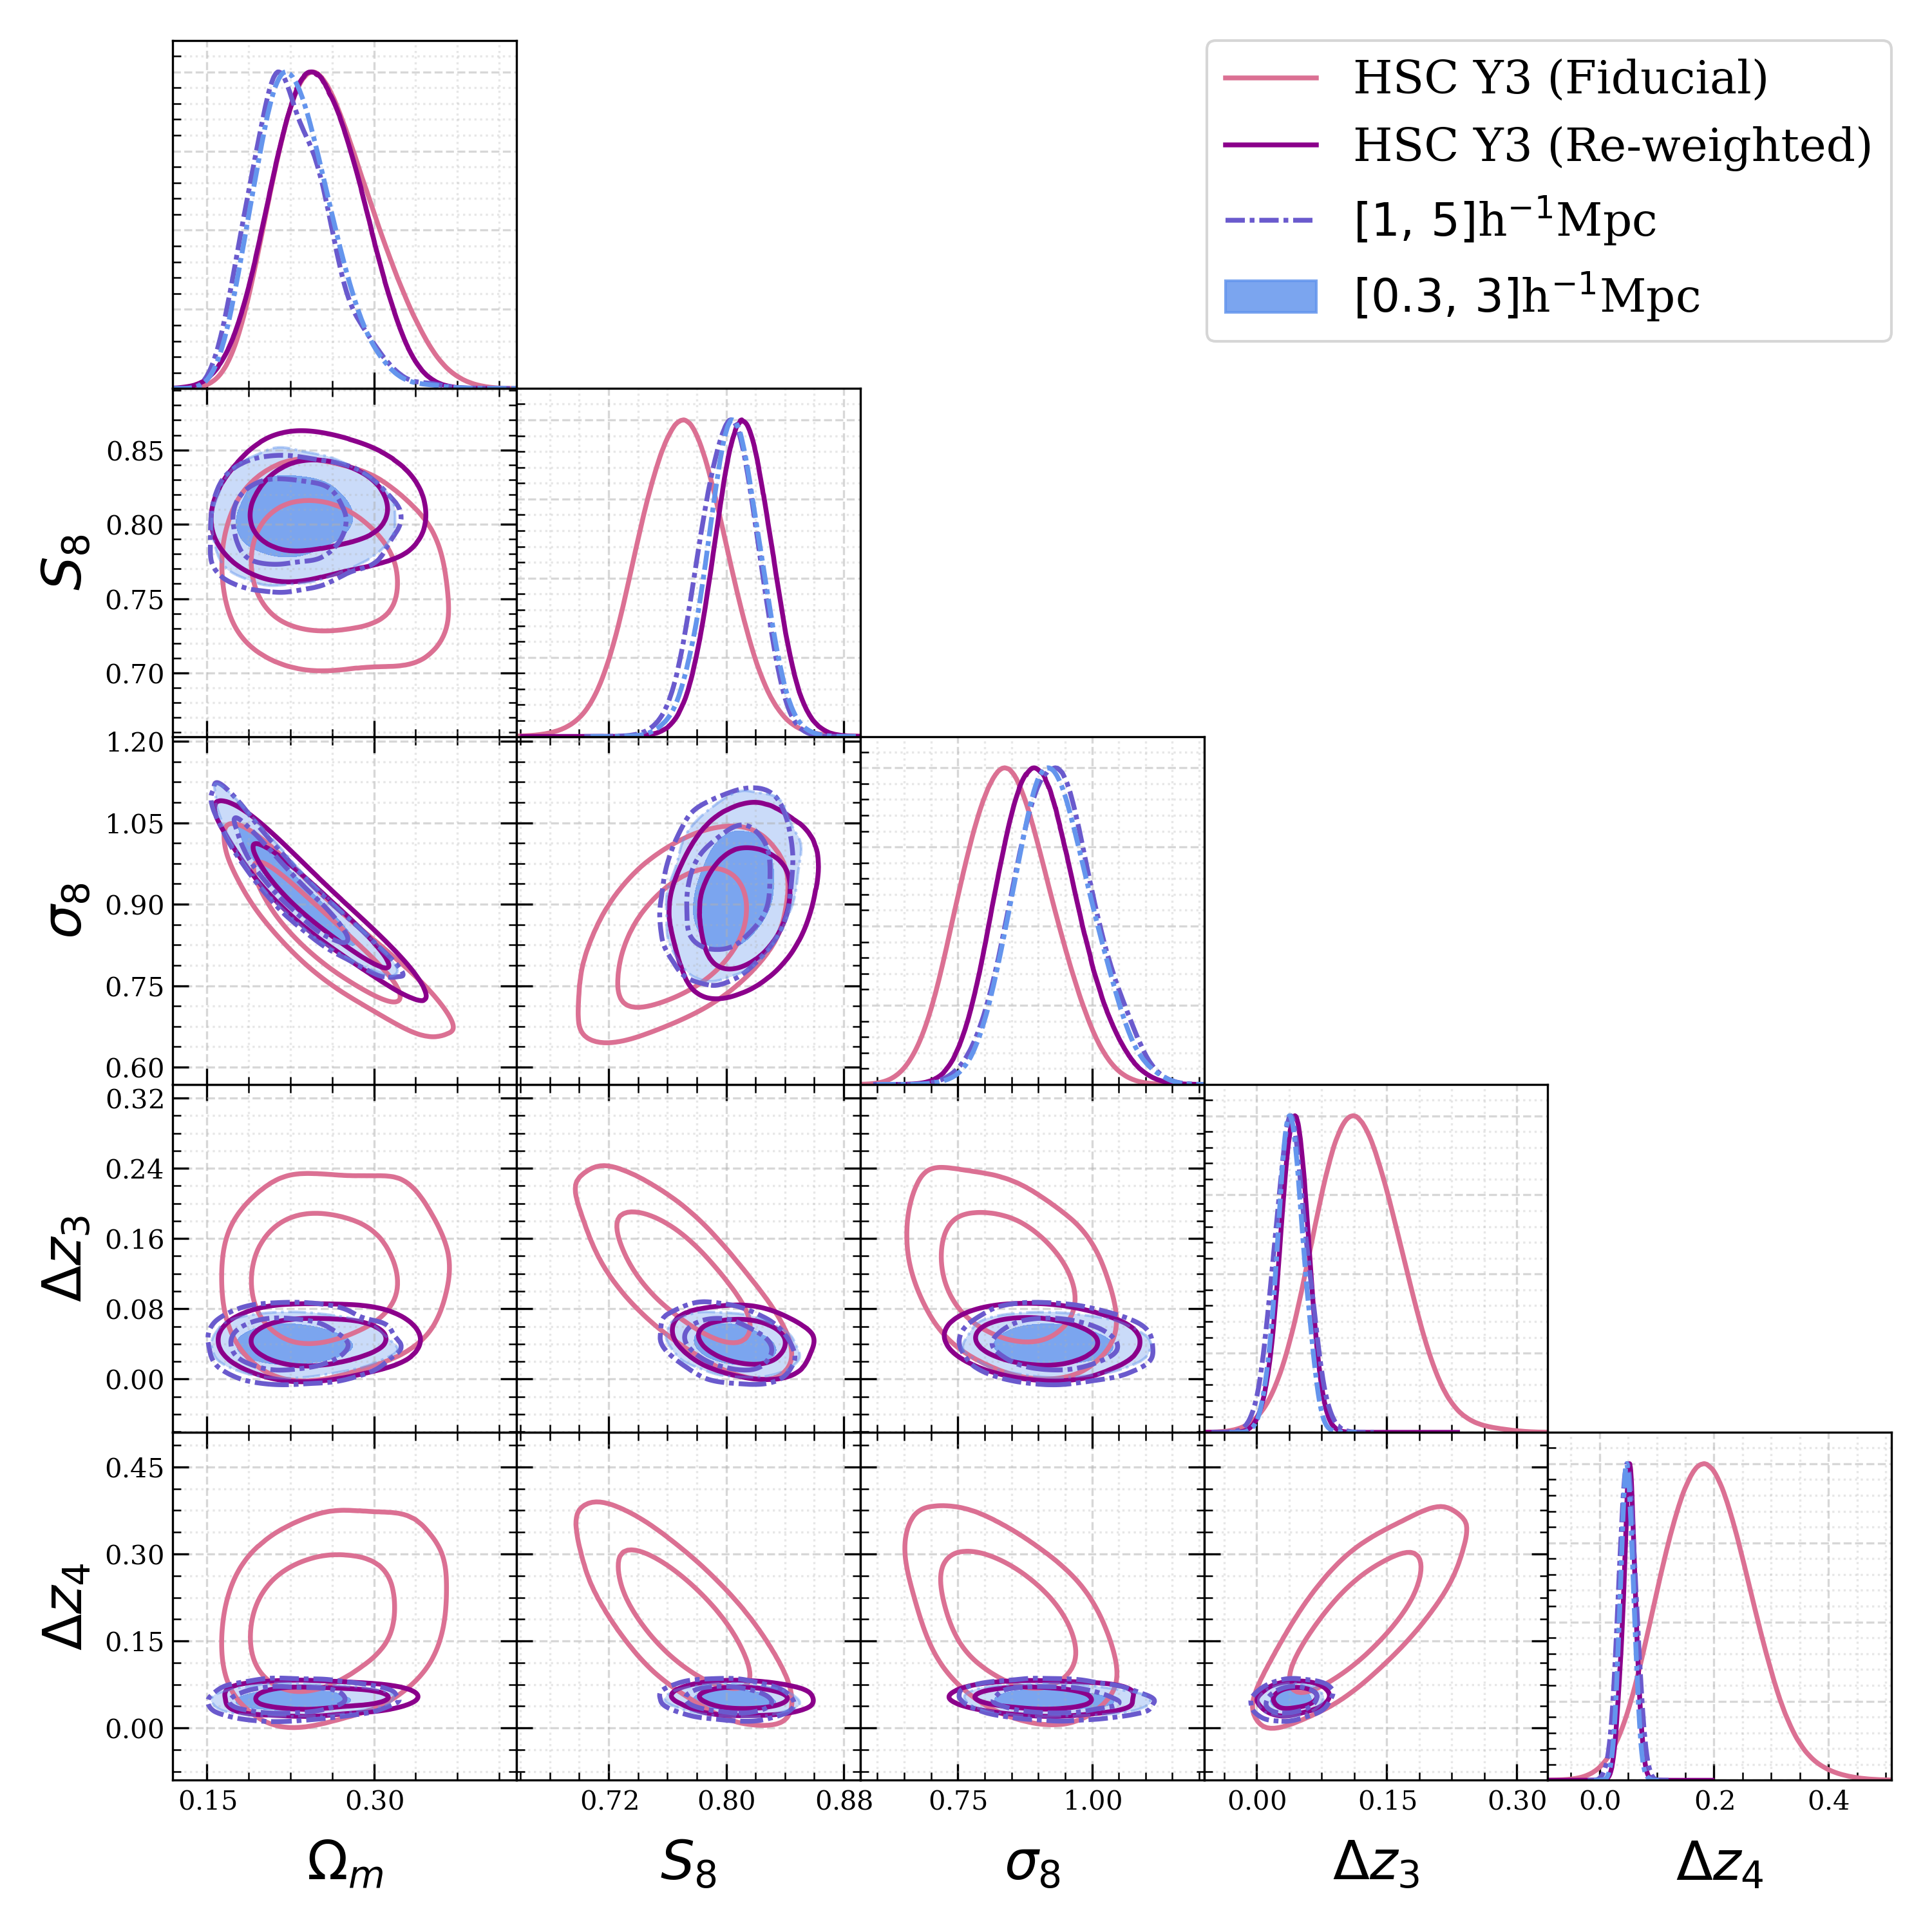
\includegraphics[width=0.95\textwidth]{img/compare_resampling_sc.png}
    \caption{Comparing the sampled results (section \ref{sec:method:mcmc}) from the two $n(z)$ set of distributions at different scale cuts with the importance re-weighting (section \ref{sec:method:importance}) approach in real space and to  the HSC Y3 fiducial result. The shift posteriors are artificially shifted by the expectation of the inferred shift in \cite{ChoppinDeJanvry2025a}, as they are by default centered around 0 for the sampling approach, since new $n(z)$ distributions are used.}
    \label{fig:corner_resampling_sc}
\end{figure}

Figure \ref{fig:corner_resampling_sc} compares the joint 2D posteriors for the fiducial result, the $1-5$h$^{-1}$Mpc scale cut $n(z)$ result to the importance sampling in real space and the fiducial HSC Y3 result. The underlying $\Delta z_{\{3,\,4\}}$ shifts lie at 1-2 sigma away from the reported posterior from the HSC Y3. While the shifts are significant in value, they are not statistically inconsistent with the self-calibration 
method deployed in HSC Y3. 

In Figure \ref{fig:corner_excluded_bins}, consistency tests are performed by running cosmological inference while removing information provided by either Bin 3 or Bin 4, and compare to the full run. The resulting corner plot displays consistent measurements between all bins. A preference towards lower $\Omega_m$ and higher $\sigma_8$ values is noticed when excluding Bin 3, akin to behavior presented in Figure 17 of the two-point correlation analysis \cite{Li2023_HSCY3_CosmicShear}, but the $\sigma$-shifts presented in Figure \ref{fig:param_sigma_shifts} alleviate concerns of inconsistencies. The lower error bound of the "No Bin 3" chain is underestimated due to the MCMC chain piling up near the boundaries of the prior ($\pi(\Omega_m)\sim\mathcal{U}(0.1, 0.7)$). Furthermore, the obtained value when excluding Bin 3 presents a fairly low value of $\Omega_m$, showing the same trend as what was obtained in the same scenario in the real space analysis \cite{Li2023_HSCY3_CosmicShear}. In this work, akin to \cite{Li2023_HSCY3_CosmicShear, Dalal2023CosmoShearHSC}, the constraint on the $S_8$ parameter is emphasized, due to the strong degeneracies between parameters $\Omega_m$ and $\sigma_8$.

\begin{figure}[ht]
    \centering
    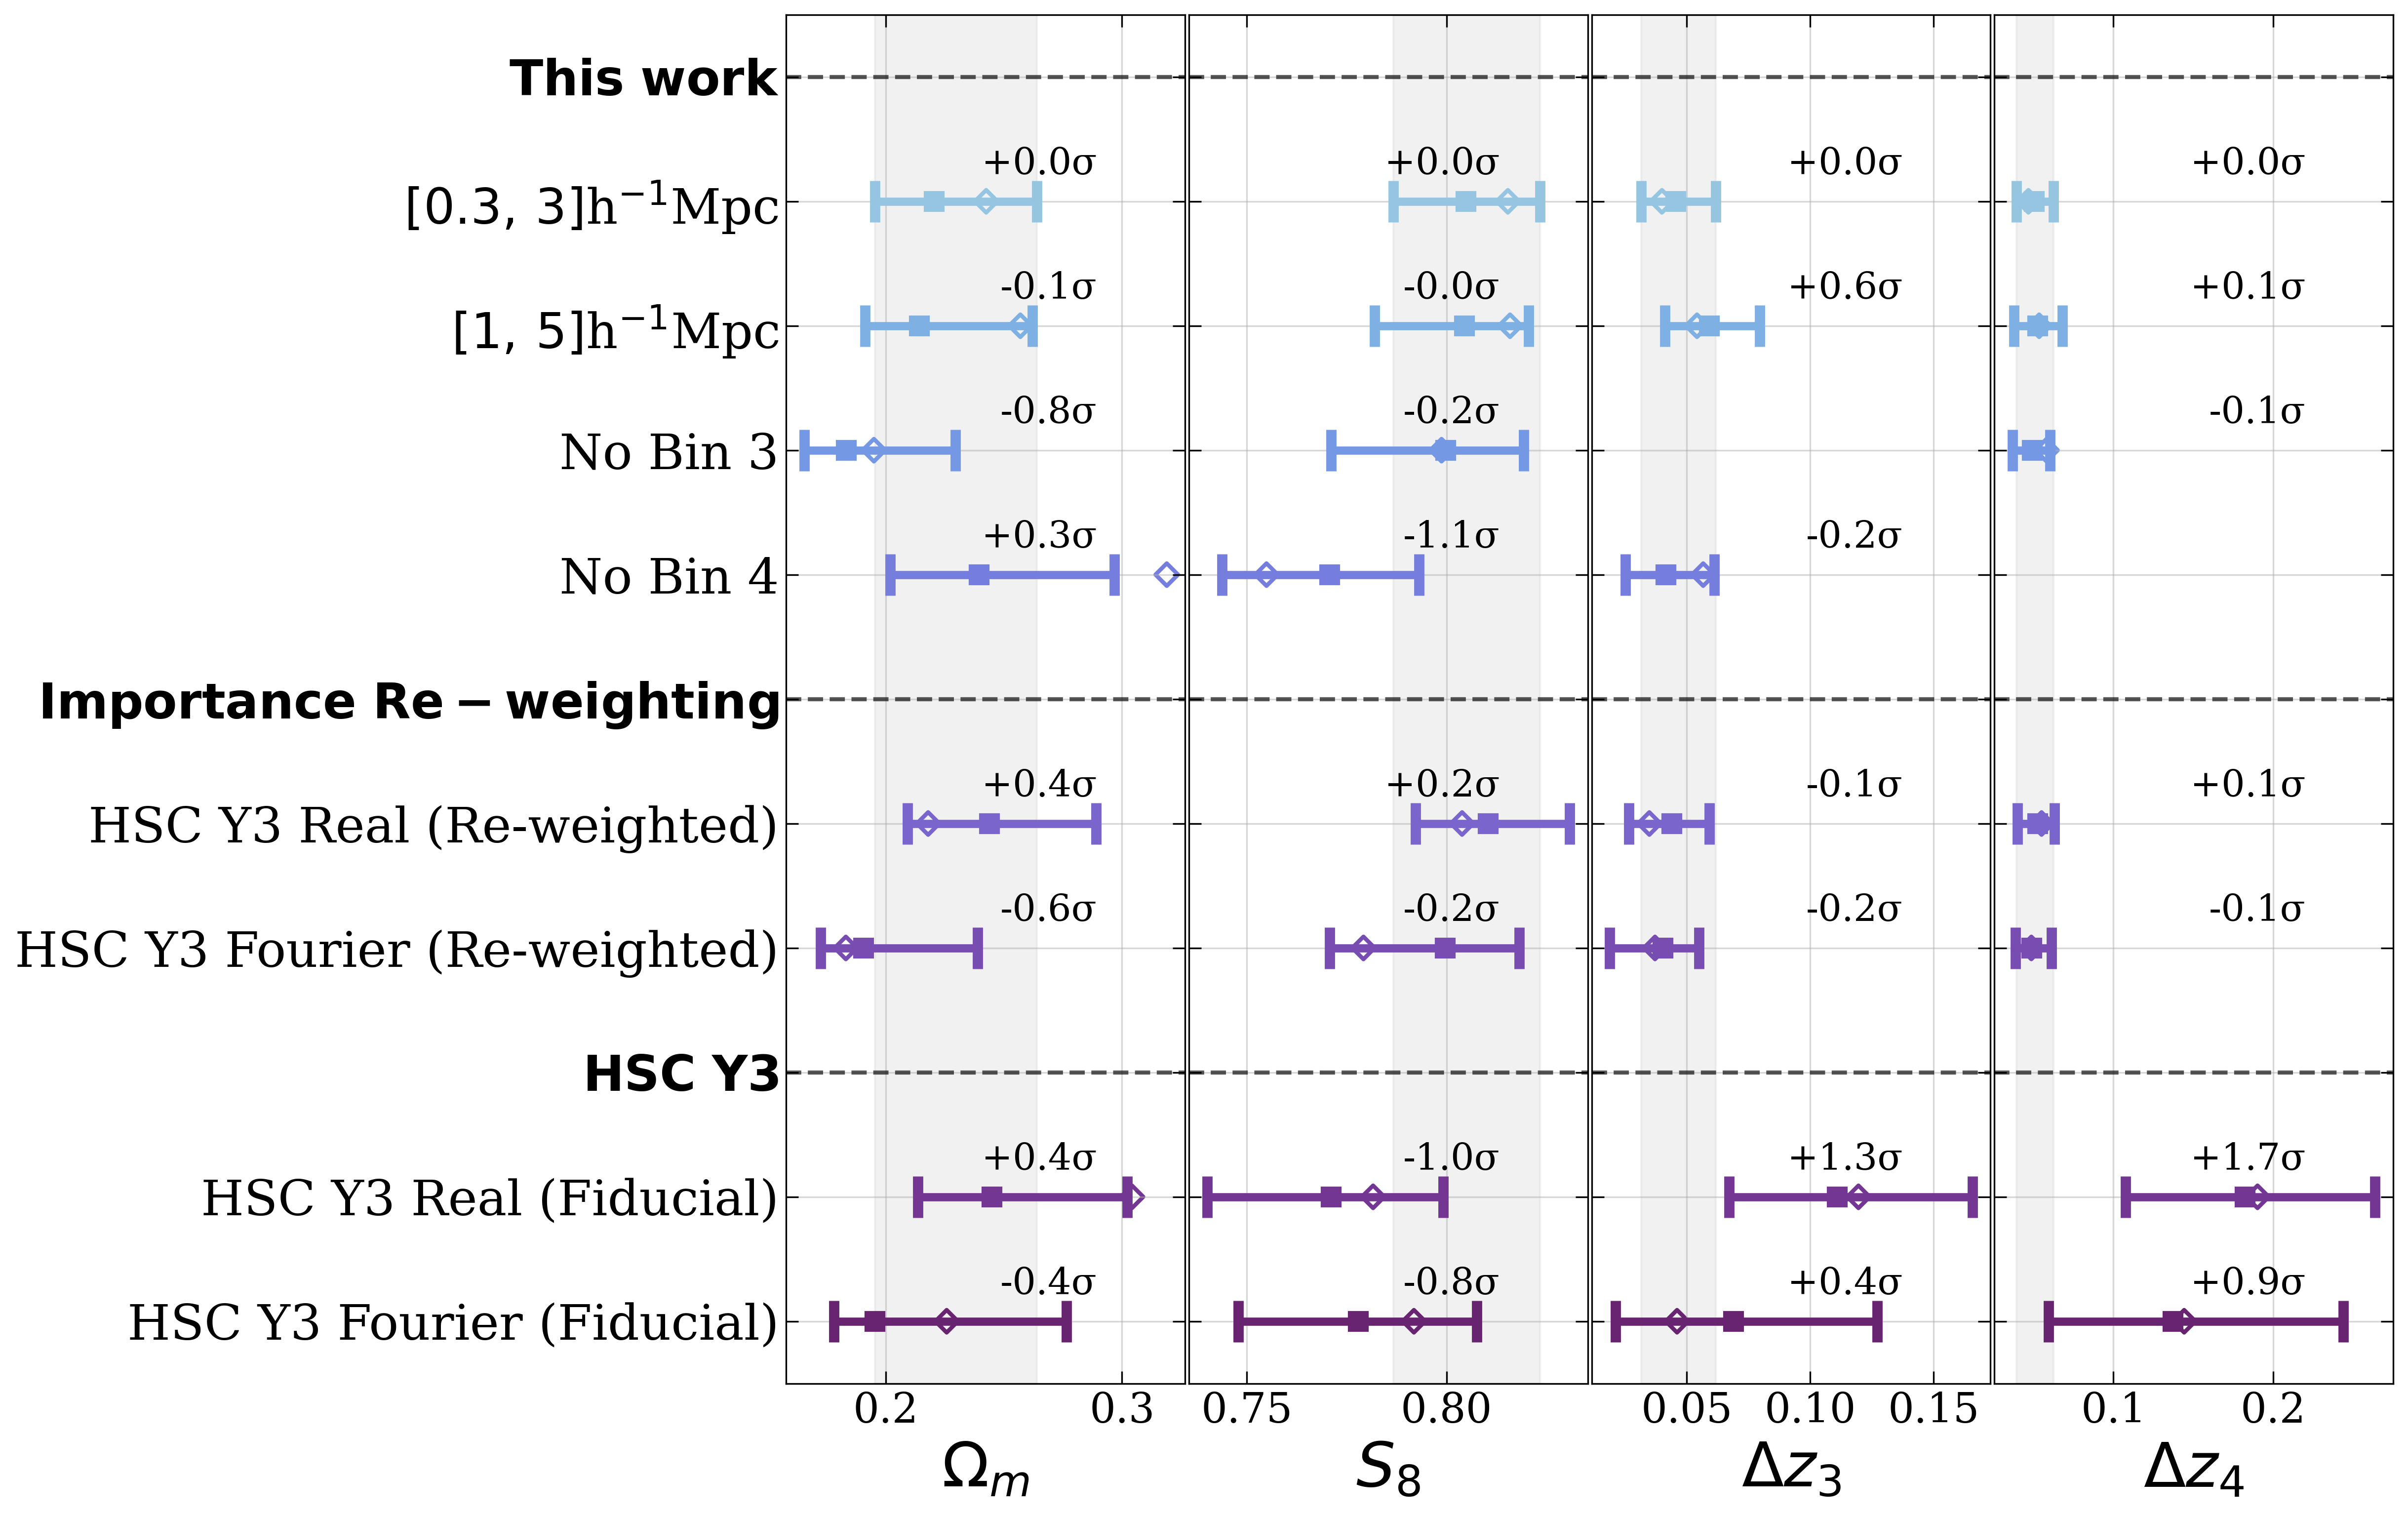
\includegraphics[width=0.95\textwidth]{img/tensions.png}
    \caption{$\Omega_m$, $S_8$, $\Delta z_3$, $\Delta z_4$ parameters compared under different measurements. This includes the sampling approach, where the $n(z)$ distributions at two different scale cuts are included, as well as the measurements obtained when excluding either Bin 3 or Bin 4. These are then compared to the importance re-weighting and fiducial results of the Real and Fourier HSC Y3 analyses \cite{Li2023_HSCY3_CosmicShear, Dalal2023CosmoShearHSC}. The square marker displays the 1D posterior mode obtained with \texttt{getDist}. The diamond marker is the Maximum A Posteriori (MAP) value. The background gray area represents the projected fiducial measurement obtained with the $0.3-3$h$^{-1}$Mpc scale cut for the $n(z)$. The $n(z)$ distributions are not the same for HSC Y3 samples (derived from \cite{HSCClusteringRau2023}) and this work (from \cite{ChoppinDeJanvry2025a}) : the posteriors of this work have been artificially shifted to match the mean of the shifts found in \cite{ChoppinDeJanvry2025a}.}
    \label{fig:param_sigma_shifts}
\end{figure}
%and the $\sigma$ deviations are computed for comparison purposes, assuming gaussian error bars with the error used being the one in the direction of the compared measurement and the distance computed over the reported modes

{\renewcommand{\arraystretch}{1.2}
\begin{table}[ht]
\centering
\caption{\label{tab:post}
Fiducial parameters and priors for this cosmological analysis. 
$\mathcal{U}(a,b)$ represents a flat (uniform) prior over bounds $[a,b]$, while $\mathcal{N}(\mu, \sigma)$ represents a Gaussian prior of mean $\mu$ and standard deviation $\sigma$. $S_8$ and $\sigma_8$ are computed quantities. The values are presented according to equation \ref{eq:presentation}. 
}
\begin{tabular}{l | l | l | l }
\hline
\textbf{Parameter} & \textbf{Prior} & $\mathbf{[0.3,\,3]}$h$\mathbf{^{-1}}$\textbf{Mpc} & $\mathbf{[1,\,5]}$h$\mathbf{^{-1}}$\textbf{Mpc} \\ 
\hline
\hline
\textbf{Cosmological Parameters} &  & & \\
$A_s\,(\times 10^9)$ & $\mathcal{U}(0.5, 10)$ & $3.721_{-0.654}^{+2.221} ({2.765})$ & $3.730_{-0.687}^{+2.410} ({2.922})$ \\ 
$\Omega_m$ & $\mathcal{U}(0.1, 0.7)$ & $0.221_{-0.025}^{+0.043} ({0.243})$ & $0.214_{-0.023}^{+0.048} ({0.257})$ \\ 
$\sigma_8$ & -- & $0.922_{-0.066}^{+0.079} ({0.907})$ & $0.936_{-0.082}^{+0.069} ({0.882})$ \\ 
$S_8$ & -- & $0.805_{-0.018}^{+0.019} ({0.815})$ & $0.804_{-0.022}^{+0.016} ({0.816})$ \\
$n_s$ & $\mathcal{U}(0.87, 1.07)$ & $0.900_{-0.005}^{+0.112} ({0.885})$ & $0.881_{--0.011}^{+0.130} ({0.898})$ \\ 
$h_0$ & $\mathcal{U}(0.62, 0.80)$ & $0.662_{-0.015}^{+0.093} ({0.746})$ & $0.701_{-0.053}^{+0.057} ({0.724})$ \\ 
$\omega_b \equiv \Omega_b h^2$  & $\mathcal{U}(0.02, 0.025)$ & $0.024_{-0.004}^{+-0.000} ({0.020})$ & $0.020_{--0.001}^{+0.004} ({0.024})$ \\ 
\hline
\textbf{Baryonic Feedback} & & & \\
$A_{\rm b}$ & $\mathcal{U}(2, 3.13)$ & $2.075_{-0.024}^{+0.695} ({2.083})$ & $2.041_{-0.054}^{+0.707} ({2.137})$ \\ 
\hline
\textbf{Intrinsic Alignment} & & & \\
$A_1$ & $\mathcal{U}(-6, 6)$ & $0.441_{-0.424}^{+0.272} ({0.648})$ & $0.432_{-0.405}^{+0.341} ({0.503})$ \\ 
$\eta_1$ & $\mathcal{U}(-6, 6)$ & $-2.478_{-1.890}^{+4.117} ({-3.549})$ & $-1.943_{-2.040}^{+3.942} ({-4.323})$ \\ 
$A_2$ & $\mathcal{U}(-6, 6)$ & $-0.058_{-0.652}^{+0.900} ({-0.603})$ & $-0.057_{-0.678}^{+0.925} ({-0.469})$ \\ 
$\eta_2$ & $\mathcal{U}(-6, 6)$ & $-1.524_{-2.330}^{+4.114} ({-3.915})$ & $-1.552_{-2.248}^{+4.352} ({-4.782})$ \\ 
$b_{\rm TA}$ & $\mathcal{U}(0, 2)$ & $0.062_{--0.117}^{+1.371} ({0.061})$ & $0.067_{--0.119}^{+1.392} ({0.163})$ \\ 
\hline
\textbf{Redshift shifts} & & & \\
$\Delta z_1$ & $\mathcal{N}(0, 0.008)$ & $-0.002_{-0.008}^{+0.008} ({-0.002})$ & $-0.003_{-0.013}^{+0.012} ({-0.004})$ \\ 
$\Delta z_1$ & $\mathcal{N}(0, 0.009)$ & $-0.002_{-0.009}^{+0.007} ({-0.009})$ & $-0.010_{-0.012}^{+0.011} ({-0.027})$ \\ 
$\Delta z_3$ & $\mathcal{N}(0, 0.020)$ & $0.007_{-0.014}^{+0.016} ({0.001})$ & $0.020_{-0.018}^{+0.020} ({0.015})$ \\ 
$\Delta z_4$ & $\mathcal{N}(0, 0.012)$ & $0.002_{-0.011}^{+0.012} ({-0.001})$ & $0.005_{-0.015}^{+0.015} ({0.005})$ \\ 
\hline
\textbf{Shear calibration} & & & \\
$\Delta m_1$ & $\mathcal{N}(0, 0.01)$ & $0.000_{-0.011}^{+0.009} ({-0.009})$ & $0.001_{-0.011}^{+0.009} ({-0.003})$ \\ 
$\Delta m_2$ & $\mathcal{N}(0, 0.01)$ & $-0.003_{-0.010}^{+0.009} ({0.001})$ & $-0.005_{-0.010}^{+0.010} ({-0.003})$ \\ 
$\Delta m_3$ & $\mathcal{N}(0, 0.01)$ & $0.000_{-0.009}^{+0.010} ({0.001})$ & $0.001_{-0.009}^{+0.010} ({-0.001})$ \\ 
$\Delta m_4$ & $\mathcal{N}(0, 0.01)$ & $0.005_{-0.009}^{+0.010} ({0.010})$ & $0.007_{-0.011}^{+0.007} ({0.005})$ \\
\hline
\textbf{PSF systematics} & & & \\
$\tilde{\alpha}_2$ & $\mathcal{N}(0, 1)$ & $0.075_{-0.988}^{+0.941} ({0.159})$ & $-0.094_{-0.819}^{+1.123} ({-0.109})$ \\
$\tilde{\beta}_2$ & $\mathcal{N}(0, 1)$ & $0.033_{-0.886}^{+1.016} ({0.160})$ & $0.102_{-1.001}^{+0.927} ({-0.120})$ \\ 
$\tilde{\alpha}_4$ & $\mathcal{N}(0, 1)$ & $-0.347_{-0.850}^{+0.993} ({-1.281})$ & $-0.271_{-0.934}^{+0.920} ({-0.461})$ \\ 
$\tilde{\beta}_4$ & $\mathcal{N}(0, 1)$ & $-0.005_{-1.066}^{+0.911} ({0.271})$ & $-0.091_{-0.971}^{+1.033} ({-0.014})$ \\  
\hline
\end{tabular}
\end{table}}

Figure \ref{fig:param_sigma_shifts} compares the relative shifts to the fiducial measurement of this work under different scenarios. We perform consistency tests with Bin 3 or Bin 4 excluded and using the distributions inferred with the larger scale cut ($1-5$h$^{1}$Mpc) obtained in \cite{ChoppinDeJanvry2025a}. The importance re-weighting results obtained with the method described in section \ref{sec:method:importance} are shown next. The measured shift in the $\Delta z$ bins in the context of the importance re-weighting, the $1-5$h$^{1}$Mpc distributions or in the context of the HSC Y3 fiducial $n(z)$ derived in \cite{HSCClusteringRau2023} cannot be strictly compared to the $n(z)$ shifts found in this work, since the $n(z)$ distributions themselves differ. Lastly, the importance re-weighting of the HSC Y3 chains means constraining the originally broad uniform $\mathcal{U}(-1, 1)$ prior over $\Delta z_3$, $\Delta z_4$ to a stricter gaussian prior. We note that reweighting leads to a fairly low number of effective sample size with respect to the original chain, leading to noisy 2D posteriors. 

\begin{figure}[ht!]
    \centering
    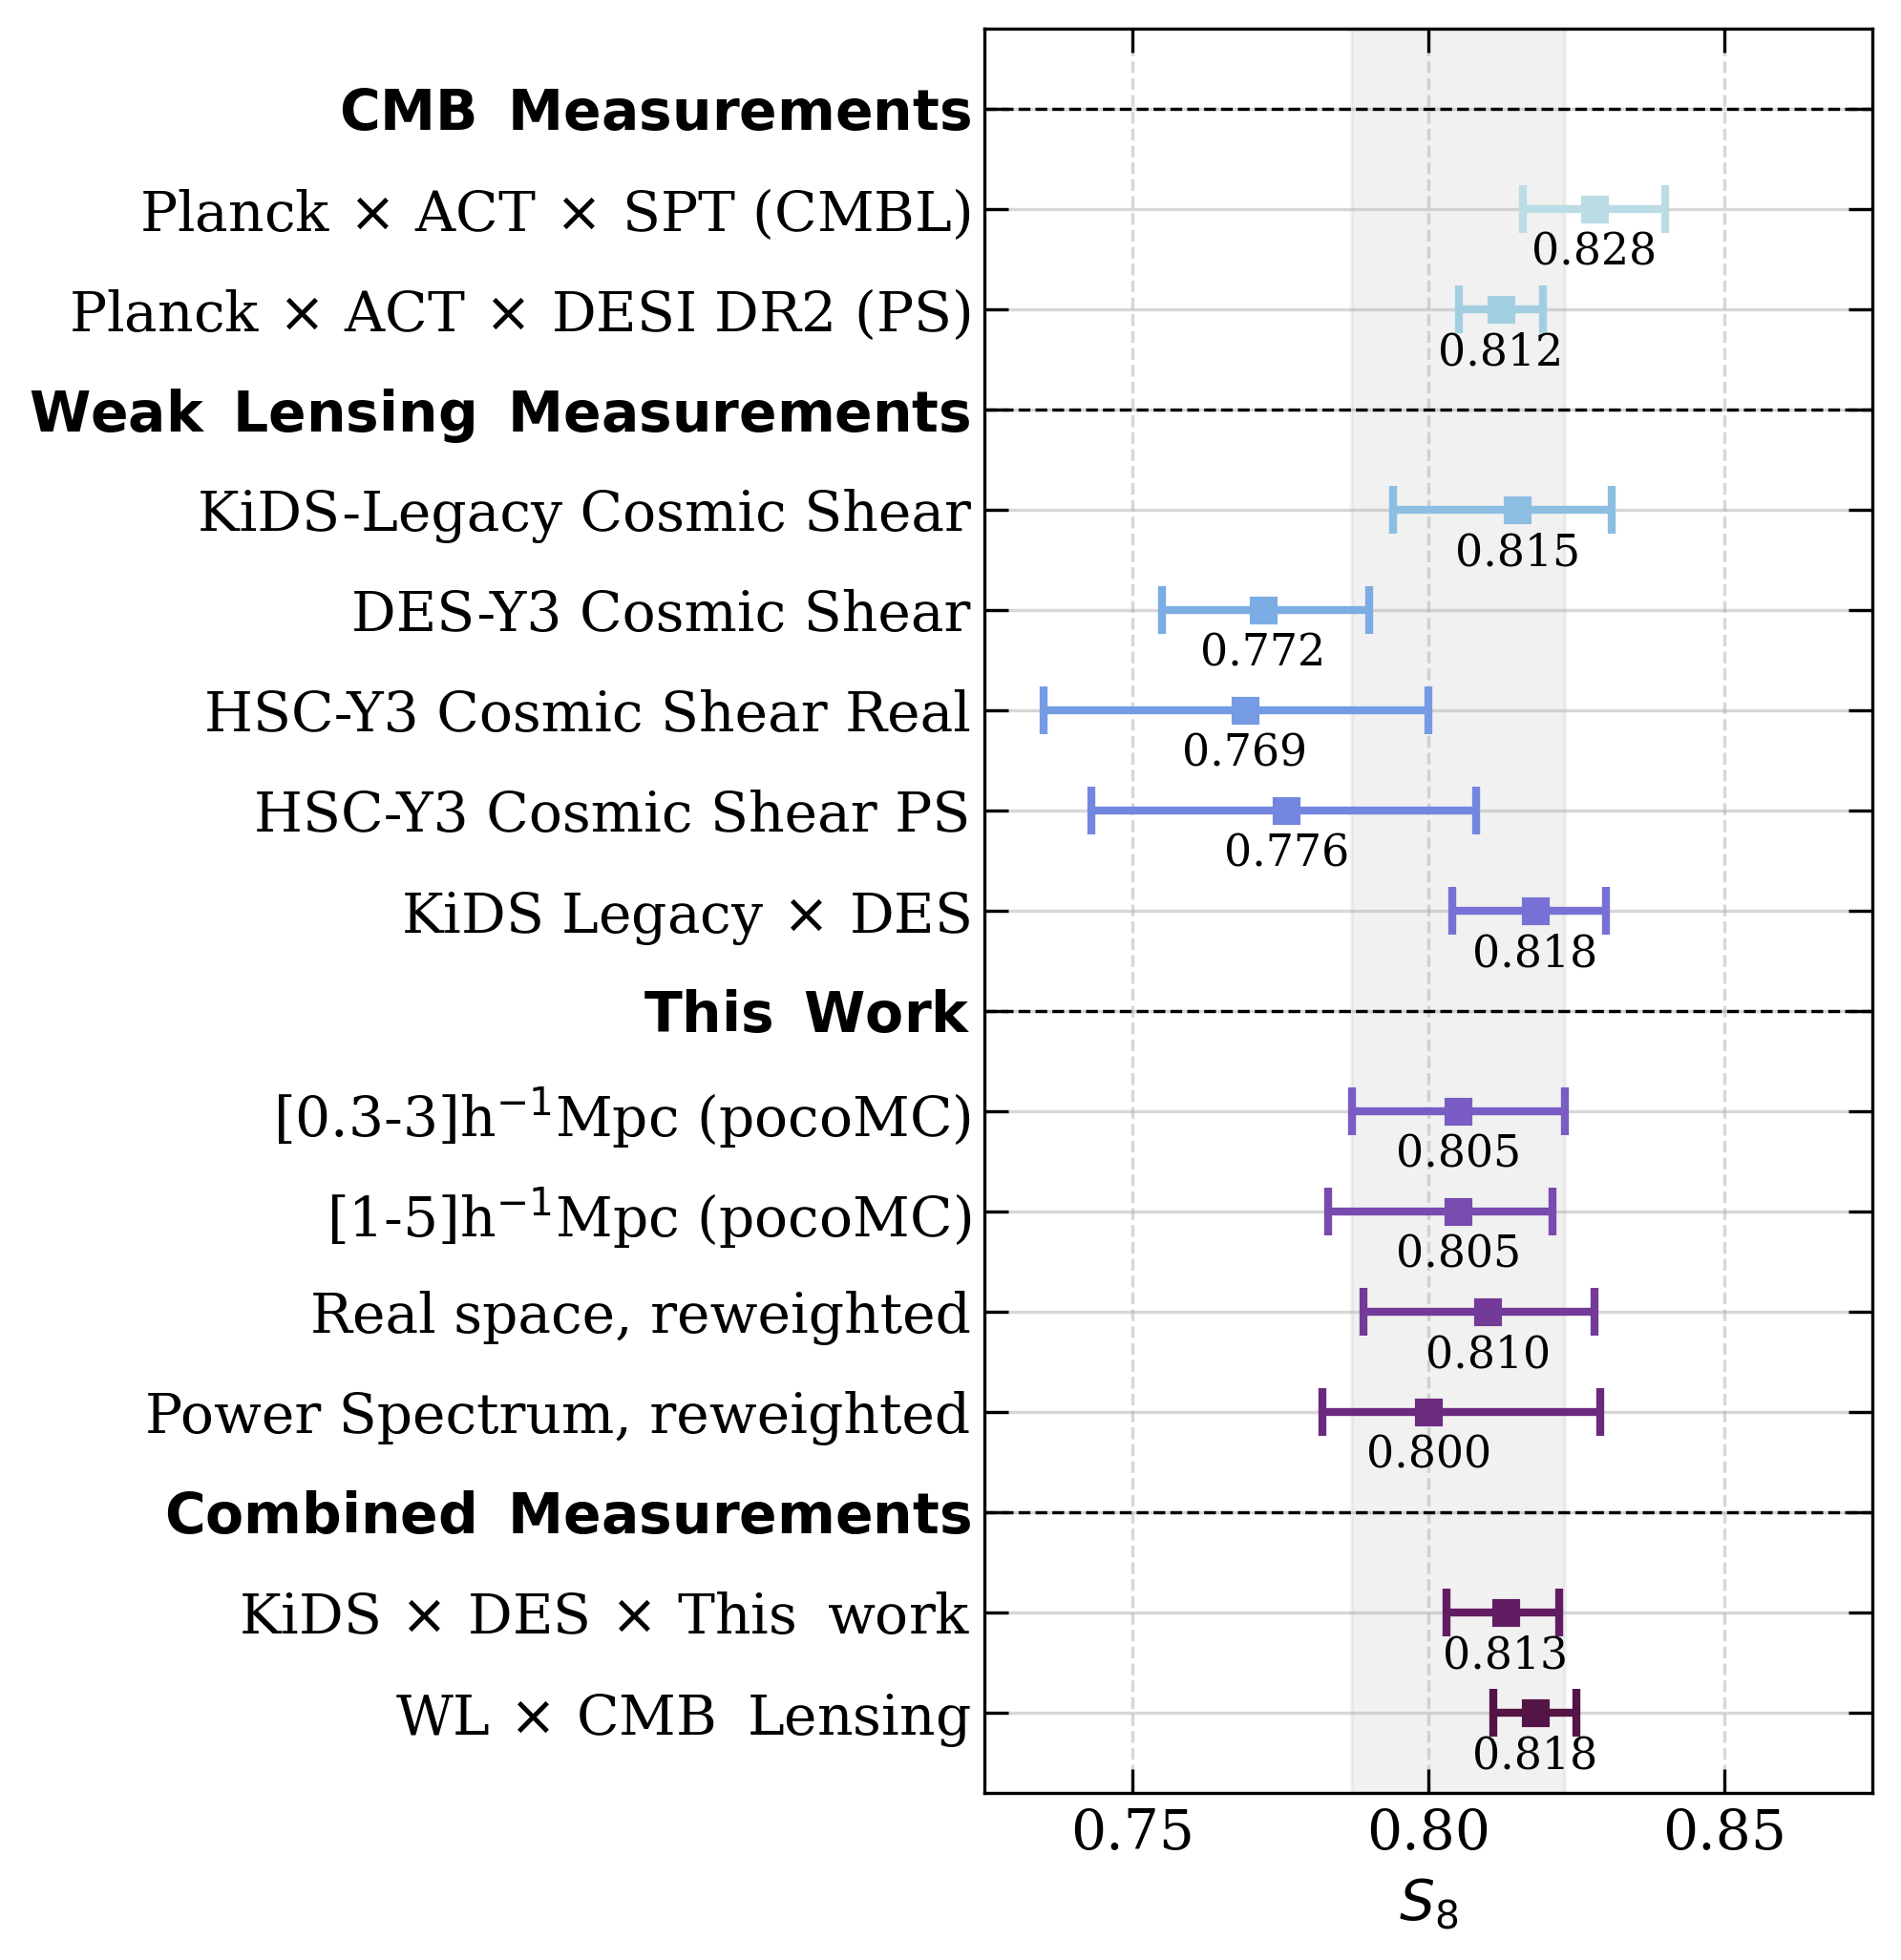
\includegraphics[width=0.95\textwidth]{img/comparison_s8.png}
    \caption{Measurements from different surveys measuring the growth of structure, from \textit{CMB Measurements} and \textit{Weak Lensing Measurements}. The results are further compared to the results obtained in this work, as well as combined with the $S_8$ constraints obtained. The  source of every cited measurement is discussed in text.}
    \label{fig:comparison_S8}
\end{figure}

The priors for all sampled parameters in the case of the fiducial $n(z)$ is reported in table \ref{tab:post}, alongside the posterior sampled values obtained for the other scale cuts. We note that the redshift $\Delta z_i$ priors depend on the chosen scale cut, as mentioned in appendix \ref{sec:appendix}.
Figure \ref{fig:comparison_S8} compares other recent $S_8$ constraints with respect to the constraints obtained in this work.  The most recent non-lensing CMB result is Planck $\times$ ACT $\times$ DESI DR2 constraints obtained from the power spectra measurements of ACT DR6 presented in \cite{Louis2025_ACTDR6_PS_S8}. The 
most recent CMB lensing result is Planck $\times$ ACT $\times$ SPT (CMBL): the CMB lensing constraints obtained from combining Planck, ACT and SPT maps in work \cite{Qu2025_ACTSPTPLANCK_CMBL_S8}.
We also show measurements obtained with weak lensing from KiDS-Legacy \cite{Wright2025_KiDSLegacy}, DES \cite{Amon2022CosmoShearDES, Secco2022CosmoShearDES}, HSC Y3 (in both real \cite{Li2023_HSCY3_CosmicShear} and Fourier \cite{Dalal2023CosmoShearHSC} space), and the combined measurement of KiDS-Legacy and DES presented in \cite{Wright2025_KiDSLegacy}. Results from this paper derived from the $n(z)$ re-calibration performed in \cite{ChoppinDeJanvry2025a} are presented next. The two scale cuts with all bins are measured with \texttt{pocoMC} sampling, as discussed in Section~\ref{sec:method:mcmc}. We also show results from importance re-weighting of the files. Finally, we combine KIDS and DES with the fiducial measurement of this work ($S_8=0.805^{+0.019}_{-0.018}\;(0.815)$) to KiDS and DES, obtaining $S_8=0.813^{+0.009}_{-0.010}$. This is further combined into the joint WL constraint with CMB Lensing information, obtaining $S_8=0.818\pm0.007$, a sub-percent constraint on $S_8$. This result can be compared to the most recent Planck $\times$ ACT $\times$ DESI DR2 ($S_8=0.812\pm0.007$), finding a similar value in both the mean and variance: we find no significant discrepancy between the two in the mean, and the combined constraining power of WL surveys is now comparable to that of the CMB.
